\documentclass{article}
\usepackage[T1]{fontenc}
\usepackage{lmodern}
\usepackage{graphicx}
\usepackage{amsmath,amssymb}
\usepackage[a4paper,margin=2cm]{geometry}
\usepackage[absolute,overlay]{textpos}
\setlength{\TPHorizModule}{1mm}
\setlength{\TPVertModule}{1mm}
\usepackage[indonesian]{babel}
\usepackage{hyperref}
\setlength{\emergencystretch}{2em}
% unit: Halaman 5

\begin{document}

% === Halaman 5 (llm) ===

\section*{1. Chipertext-only attack}

Kriptanalis hanya memiliki cipherteks saja. Ini serangan paling sulit karena informasi yang diperoleh hanya sedikit (cipherteks saja).

Teknik yang digunakan: \textit{exhaustive key search}, terkaan, \textit{metode} analisis frekuensi, dsb.

Diberikan: \[ C_1 = E_k(P_1), \quad C_2 = E_k(P_2), \quad ..., \quad C_i = E_k(P_i) \]

\vspace{71.28mm}

Deduksi: \[ P_1, P_2, \dots, P_i \text{ atau } k \text{ untuk mendapatkan} \]
\[ P_{i+1} \text{ dari } C_{i+1} = E_k(P_{i+1}). \]

\vspace{10mm}

% deskripsi: Diagram ilustrasi serangan Ciphertext-Only Attack yang menunjukkan Alice mengirim ciphertext ke Bob, dan Eve mencegat ciphertext tersebut untuk dianalisis guna mendapatkan plaintext.
% bbox normalisasi: [0.5200, 0.6300, 0.9800, 0.8700]
\begin{textblock*}{96.60mm}(109.20mm,187.11mm)
\noindent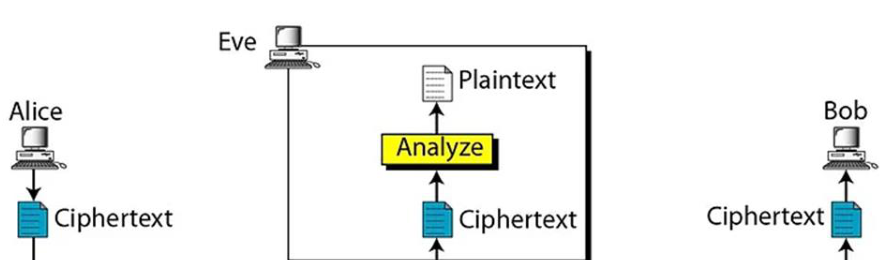
\includegraphics[width=96.60mm,height=71.28mm]{../../images/llm/page_005_img_01.png}%
\end{textblock*}

\end{document}
